\documentclass{ucl_thesis}

%twoside for double page printing
\usepackage{enumerate}
\usepackage{graphics}
\usepackage{graphicx}
\usepackage{color}
\usepackage{verbatim}
\usepackage{algorithm}
\usepackage{algorithmic}
\newcommand{\theHalgorithm}{\arabic{algorithm}}

\usepackage{listings}
\usepackage{amsmath}
% Uncomment this to activate the TikZ library, which is useful for fancy block-diagrams.
%    \usepackage{tikz}
%    \usetikzlibrary{positioning,arrows,shapes.misc}
\usepackage{multirow}

%\numberwithin{algorithm}{chapter}
%\usepackage{epsf}
\usepackage{fancyvrb}

% Uncomment this package to enable internal-linking:
%\usepackage{hyperref}


\title{``Scan to search''\\
        A 3D retrieval system}

\author{Mincong Zhang}
\def \supervisor {Dr Seena Rejal(3DI); Dr Niloy Mitra (UCL)}

\date{September 2014}


%Malcolm added some custom commands here - you can make your own!
\newcommand{\vect}[1]{\boldsymbol{#1}}
\newcommand{\figref}[1]{(Fig. \ref{#1})}

% See this one in use further down:
\def\etal{{et~al.}}

% I also like these, but didn't have occasion to use them below:
\def\ie{{\it i.e.,\ }}
\def\etc{{\it etc.,\ }}
\def\eg{{\it e.g.,\ }}
\def\vs{{\it vs.\ }}


%\renewcommand{\baselinestretch}{1.5}
%\renewcommand{\bibname}{References}




\begin{document}
\bibliographystyle{abbrv}
\maketitle
\numberwithin{algorithm}{chapter}
\setcounter{page}{1}
\pagenumbering{roman}
\pagestyle{plain}

% Notice how the star "*" is used throughout LaTex to modify the normal behavior. For example, \section* instead of \section 
% tells LaTex NOT to number this section.


\newpage
\section*{Abstract}
%abstract content
As the amount of 3D data is increasing on the Internet, many kinds of 3D retrieval engines are developed. Basic keyword-based retrieval techniques are not always effective, therefore content-based retrieval engines appear. This project focuses on developing a shape-based retrieval system, which provide a "scan to search" solution for manufacturing components. The user can scan a object and reconstruct its 3D model with an app "123D", and use the scanned 3D point cloud to retrieve models with similar shape. 

Firstly, the scanned data needs to be pre-processed. Scanning noise will be reduced via a 3D bilateral filter. Then the 3D data will be rasterized to a voxel grid and normalized to a certain scale. Thus high frequency noise is avoided while the shape information is mostly kept. Secondly, the shape information is described by applying a spherical harmonics decomposition of 3D data, as well as computing a distances distribution. These describtors are rotation invariant and noise insensitive. By computing the Euclidean distance between two descriptors, the similarity of two 3D models can be acquired, and thus the system can retrieve models with similar shapes. Also, this system provides six candidate models with high similarities, so that to avoid mis-matching. 

To verify the system, a series of tests are carried out. Rotational invariance are first tested to verify that the rotation invariant descriptors are computed correctly. Noise resistant test is then carried out. The last test is to input a scanned 3D model, and retrive similar models in the database. The results are analysed. According to the results, some adjustments are made for more precise matching. 


\newpage
\section*{Acknowledgements}
I would like to express my deep gratitude to Dr Seena and Dr Niloy, my project supervisors, for their patient guidance, enthusiastic encouragement and useful critiques of this project. 

I would also like to extend my thanks to the technicians of Dr Seena's company,Patrick Min and Emanuel Geromin, for their technical support and their help in offering me data to test my program.



%\setcounter{tocdepth}{2}
\tableofcontents
\listoffigures
%\listoftables
\listofalgorithms
\newpage

%\clearpage
%
%\begin{center}
%\textbf{To whomever}
%\end{center}





\setcounter{page}{1}
\pagenumbering{arabic}
\pagestyle{plain}

\chapter{Introduction}
\label{background}

%Introduction
%First and foremost, you should write about the most interesting or important parts of your project. Devote most space and time to this. For example:

 

%    What design choices did you have along the way, and why did you make the choices you made?
%    What was the most difficult part of the project?
%    Why was it difficult?
%    How did you overcome the difficulties?
%    Did you discover anything novel?
%    What did you learn?


%Set the scene and problem statement/specification. Provide the motivation for reading this report. Introduce the structure of report (what you will cover in which chapters). 


%How to write introduction: 
% http://www.ldeo.columbia.edu/~martins/sen_sem/thesis_org.html
\section{Introduction of the project}

With the development of 3D construction techniques, the number of available 3D models on the Internet is increasing. This makes the challenges change from construction to retrieval. A basic approach to retrieve data is keyword-based retrieval. However, this simple approach often fails for 3D data. Therefore, content-based 3D retrieval engines are developed and have been used. 3D retrieval engines can be used in many domains such as entertainment, medicine, education, and industry field. These domains have a growing demand of 3D models, it is much efficient for them to find and reuse a 3D model rather than construct a model which may already exist. 

This project tries to help the company 3DI to implement a prototype of shape-based retrieval system, which provides a ``scan to search'' solution. The company 3DI wants to connect customers and suppliers of manufacturing components through a 3D retrieval system. The user can scan a object and reconstruct its 3D model, and this system takes the scanned point clouds of manufacturing components as queries, and search for 3D models with similar shape. This is similar to content-based similar image retrieval engine provided by Google. 

However, how to choose an appropriate method to describe the 3D data and retrieval become a question. Researchers have designed lots of algorithms to describe the 3D content. In these algorithms, descriptors are the data that can representing certain features of the model. By extracting one or multiple of these descriptors from two models, matching algorithm can be carried out and determine whether the two data are similar. For different purposes different types of 3D retrieval engines are developed. For example, the shape-based retrieval engines use a 3D data as query to find models with similar shapes. While the sketch-based 3D retrieval engines can help people who has no reference model but an idea, to draw sketches and search. Another retrieval engines may extract metadata from 3D models and used as a matching feature. The details of these matching algorithms are discussed in Chapter~\ref{background} Section~\ref{sec:3dretrieval} and Section~\ref{sec:retrievalalgorithms}. 

For this project, it is important to choose an appropriate type of descriptors to describe the query model. Since the query model is reconstructed by scanning, it contains scanning noise, which may have influence to the matching algorithm in retrieval. Also, the scanned model cannot be guaranteed to align with the axises properly, i.e., the model may be rotated to any direction. Therefore, the descriptors should have rotation invariant property. After investigating the algorithms for describing and matching 3D models, a suitable descriptors is chosen for this project - the spherical harmonics shape descriptors~\cite{kazhdan2003rotation}. Comparing with other descriptors, the spherical harmonics descriptors are rotation invariant and insensitive to noise. Therefore, spherical harmonics descriptors are chosen in this ``scan to search'' retrieval system. Chapter~\ref{background} Section~\ref{sec:designchoice} shows the details of this design choice. Chapter~\ref{background} Section~\ref{computational_techniques} discusses the computational techniques of the spherical harmonics and its rotation invariant property. 

With the chosen descriptors, the next step is to design the system. Before computing descriptors, a denoising module is implemented. Although the spherical harmonics are resistant to noise to some extent, the denoising module is used if the scanned model contains high level of noise. Then comes the pre-processing. Pre-processing steps includes rasterization and normalization. Afterwards, descriptors are able to compute. To overcome the potential inaccuracy of the results, the system will show six candidates model with high similarities to the input model. The detailed analysis and design are in Chapter~\ref{chp:analysis&design}. Chapter~\ref{chp:impl} provides the implementation details of the system. 

The system will not be complete without testing. Chapter~\ref{chp:analysis&design} also discusses how to carry out several tests in every stage of implementation. For example, rotation invariant test is to verify the correct implementation of the descriptors' computation. ``Scan to search'' test is to verify the system can work with real scanned models. An interesting discovery from the tests is that the spherical harmonics tend to have numerical errors in some circumstances (e.g. a model with unusual shape). Thus another simpler descriptors distance histogram are added for assistance and compensate these errors. The analysis details are in Chapter~\ref{chp:test&results} and Chapter~\ref{chp:conc}. The final results analysis and conclusion are also in Chapter~\ref{chp:test&results} and Chapter~\ref{chp:conc}. In summary, with single spherical harmonics the retrieval results sometimes have irrelevant matches. But with the assistance of a new descriptors, the ``scan to search'' 3D retrieval system works very well. 

\section{Discussion of challenging parts}

During the implementation, there are some interesting (or challenging) parts worth discussing. The first part is try to make the pre-processing efficient. And the rasterization step can be explored. Rasterization is to sample the 3D model into a voxel grid. However, to rasterize, a $2R\times2R\times2R$ voxel grid is created, where $R$ is normally set as 32. So the size of the voxel grid is $2R\times2R\times2R = 262144$, which may occupy a huge memory space. So it is necessary to find a method, which can both save memory and compress the computational complexity. 

The idea is to save each voxel information in bit, so that to use minimum memory space. One approach is to create a temporary bitmap (bitset or boolean array in C++) of length $2R\times2R\times2R$ to record whether a voxel is filled. Each element of this bitmap can only show 1 or 0 (true or false), so that the whole bitmap will not occupy any redundant space. While in one traversal($O(n)$) of surfaces of the model, the voxel grid will be filled and the grid vertices should be stored. The implementation details are in Chapter~\ref{chp:impl}. 

The second challenging part is to understand and implement spherical harmonics decomposition. At first the transformation is implemented incorrectly, and the rotational invariance test does not pass, due to the wrong spherical harmonics decomposition. After reimplementing and testing, the final decomposition shows rotation invariant property and thus the spherical harmonics are correctly implemented.  Actually the spherical harmonics are like Fourier transform in 3D, whose coefficients show the feature of the decomposed function in space. And the energy ($L_{2}$-$norm$) of these coefficients can be used to represent the 3D shape information. Chapter~\ref{background} Section~\ref{computational_techniques} discusses these computational techniques.

Besides, spherical harmonics decomposition is time-consuming. However, due to the time limitation of this project, a fast spherical harmonics decomposition has not been investigated. This method is saved for the future work of Chapter~\ref{chp:conc}.

\chapter{Background}
\section{The area of 3D retrieval} \label{sec:3dretrieval}

With the development of 3D construction techniques, such as new multimedia softwares, interactive tools, 3D scanners and 3D printers, the number of available 3D models on the Internet is increasing. Many domains such as entertainment, medicine, education, and industry field have a growing demand of 3D models, it is much efficient for them to find and reuse a 3D model rather than construct a model which may already exist. This development in 3D field makes the challenges change from construction to retrieval. A basic approach to retrieve data is keyword-based retrieval. However, this simple approach often fails for 3D data. For example, if a 3D model is named as ``1.stl'', both the system and the user can never know its content. Besides, even with keywords, it is difficult to describe a 3D data properly because of the ambiguity in language. 

Therefore, content-based 3D retrieval engines are developed and have been used. Different types of 3D retrieval engines are used in different situations. For example, if the user has an original 3D model and want to find other similar 3D models, the shape-based retrieval system will be helpful~\cite{Funkhouser:2003:SEM:588272.588279}; but if the user has no data to describe what he/she wants to search, and just has an idea about what kind of model does he/she want, sketch-based 3D retrieval will be better~\cite{CGF:CGF12200}. 

\section{Retrieval algorithms} \label{sec:retrievalalgorithms}

Lots of algorithms are developed to describe and match the feature of 3D data. In these algorithms, descriptors are the data that can representing certain features of the model. By extracting one or multiple of these descriptors from two models, matching algorithm can be carried out and determine whether the two data are similar. With reference 3D models (or sketch data), there are many approaches to match them with the candidate models in the database. 

For sketch-based retrieval, one approach is to use 3D sketch as a query to retrieve a similar model, such as the ``Teddy'' by Igarashi~\etal~\cite{Igarashi:2007:TSI:1281500.1281532} and the ``Sketch'' by Zeleznik~\etal~\cite{Zeleznik:2007:SIS:1281500.1281530}. However, the accuracy of the results does not only lie in the robustness of matching algorithms, it also depends on the sketching skill of the user. It is difficult for most users to draw proper sketch for the system to recognize and process. This will increase the processing burden of the system, while make the accuracy of the result decrease. Additionally, the user also need some time to learn to use this kind of drawing interface. 

2D sketches in different views of object are considered as another approach. T. Funkhouser~\etal~\cite{Funkhouser:2003:SEM:588272.588279} provides a solution on 2D sketch based retrieval. In this approach the user only needs to draw 2D projections (usually three orthographic views) of a 3D model. Drawing 2D sketches is easier than 3D sketches, and the interface is much easier for users to learn.  

Recently one another approach by Xie~\etal~\cite{CGF:CGF12200} combines the advantages of the previous 2D and 3D sketches. In their approach the user can draw sketches on the 2D projection of the 3D model, which is interactively updated as the 3D model rotates. It also supports partial object retrieval, and the result can then be combined and assembled to the original object. 

For shape-based 3D retrieval, different approaches focus on exploring different features (descriptors) for object recognition, such as shock graphs~\cite{siddiqi1999shock}, medial axes~\cite{bardinet2000structural}, topology matching~\cite{hilaga2001topology}, skeletons~\cite{sundar2003skeleton}, 3D histogram~\cite{belongie2002shape} and 3D context~\cite{belongie2001matching}. 

3D histogram is one kind of statistical descriptors; it is able to describe the shape context of a 3D object. According to the approach by S. Belongie~\etal~\cite{belongie2001matching}~\cite{belongie2002shape}, the 3D model should be firstly move to its centre of mass. By creating certain voxel grid in space, the number of grids the surface come across is then computed. Therefore the polar histogram in 3D space is created. The advantage of this approach is that the shape context can be easily acquired, and the shape matching can be quickly carried out by searching for shape similarity in the 3D histograms. Also to some extent, the result is robust to noise. However, further processing is required, because the histogram created by this approach will change when the object is rotated. 

Extracting topological information like skeletons is also an approach to carry out shape-based retrieval. H. Sundar~\etal~\cite{sundar2003skeleton} encodes geometric and topological information of 3D models in skeletal graph, so that to measure similarities between 3D models. In this approach firstly transfers the 3D mesh into voxel representations, and then apply an algorithm called Parameter Controlled Volume Thinning by Gagvani~\etal~\cite{gagvani1999parameter}, to acquire the skeletal points. These skeletal points will be connected in an undirected acyclic shape graph. And the graph will be decreased to a denser skeletal graph by minimum spanning tree algorithm. By applying different values of thinness parameter, the hierarchical graph structure can be obtained. The similarities between models are able to be measured by comparing their hierarchical graph structures. 

But these approaches are time-consuming and sensitive to small features. Kazhdan~\etal~\cite{kazhdan2003rotation} uses spherical harmonics to describe shapes and match models. This approach is also applied in a 3D retrieval engine by T. Funkhouser~\cite{Funkhouser:2003:SEM:588272.588279}. The main steps is shown in Figure~\ref{background_sphericalharmonics}. Firstly a voxel grid is created; a binary function is used to represent whether the voxel grid contains the surface of the 3D model.  The results need to be normalized so that to have a unit length from the centre of mass to the average distance from every voxels. These steps make sure the data are scale invariant and high frequency noise can be removed. The next step is to transfer voxels to spherical coordinates so that to obtain the spherical functions. By decomposing the spherical functions, spherical harmonics can be acquired. For each frequency, they add up the harmonics and compute their energy, and then the rotation invariant signature can be acquired. For different radii sum up the different signatures, the spherical harmonics descriptor for 3D data can finally be computed. The result will be a 2D histogram, representing the radius and frequency. Thus it is invariant to rotations. Also because the dimensionality of the descriptor is 2D, this approach will be more efficient in comparing and matching models. And therefore this approach is good for large database. However, its limitation is that it cannot detect models which are different in interior rotation. 

\begin{figure}[h]
\centering
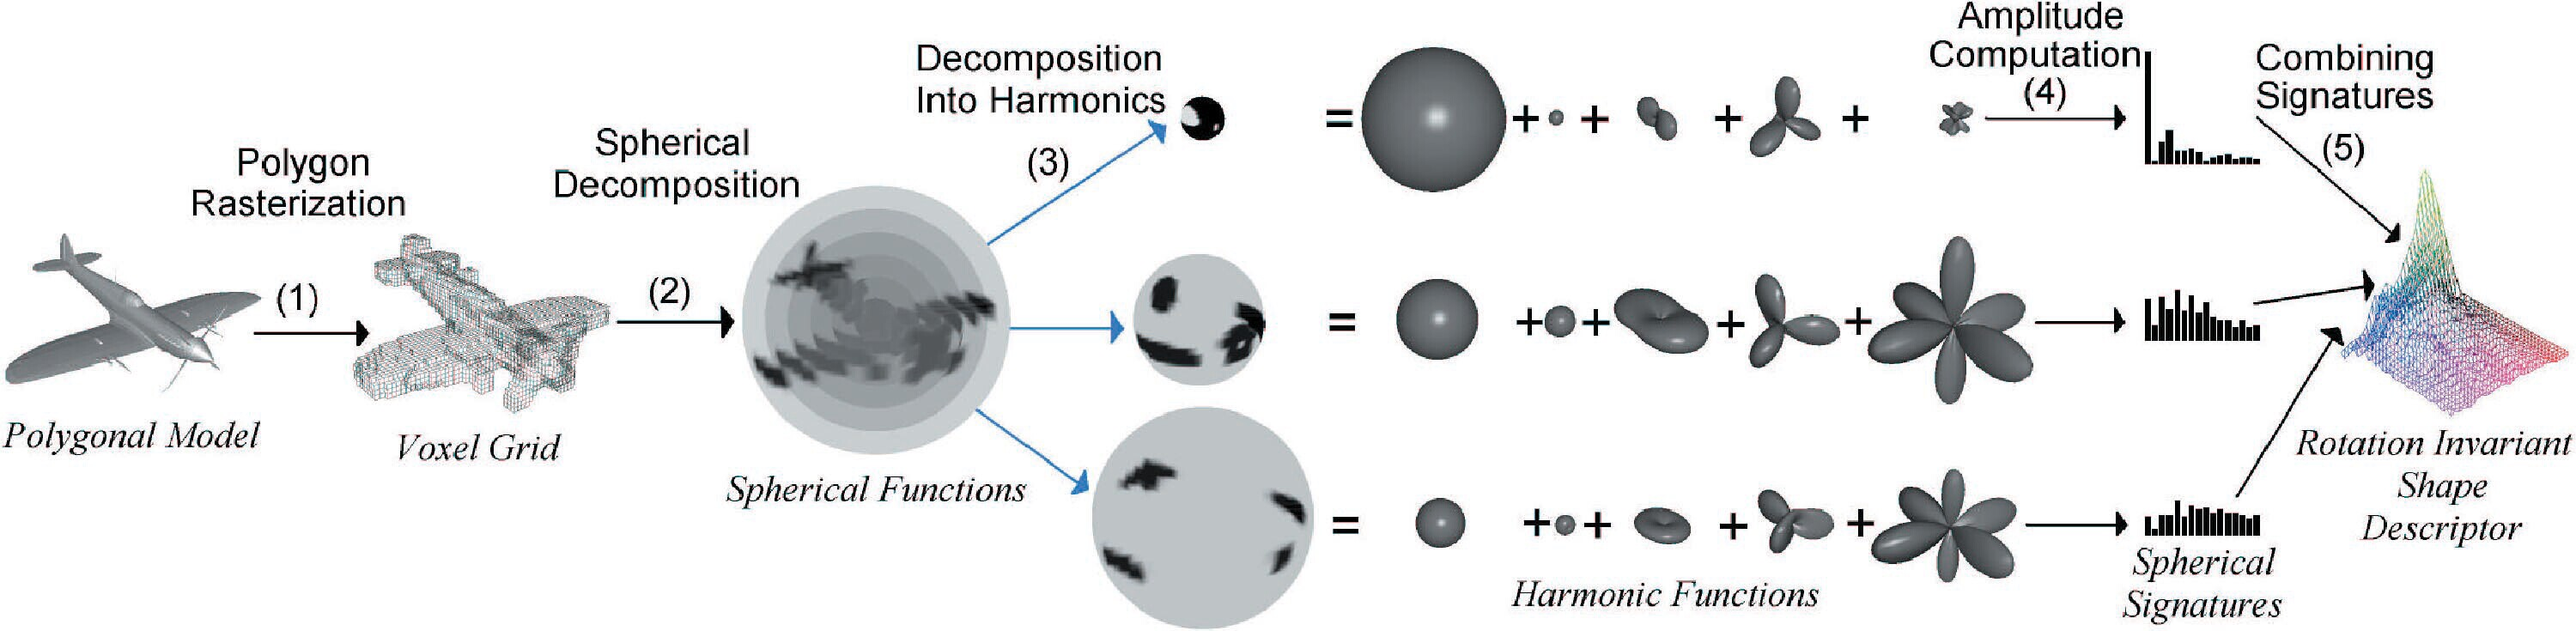
\includegraphics[width=0.9\linewidth]{background_sphericalharmonics}
\caption{Computing spherical harmonics shape descriptor~\cite{Funkhouser:2003:SEM:588272.588279}} \label{background_sphericalharmonics}
\end{figure}


With certain retrieval method, the search engine can be built. Many universities and research institutions have developed their 3D retrieval engines, such as the 3D model search engine at the Princeton University~\cite{shilane2004princeton}~\cite{min2003early}, the 3D model retrieval system at the National Taiwan University~\cite{shen20033d}, and the Purdue University~\cite{iyer2005engineering}. Besides, database and benchmarks are required, for process the search engine as well as testing the search algorithm. The first benchmarks for 3D mesh models is created by Princeton University~\cite{shilane2004princeton}. There are 1, 814 models in the Princeton Shape Benchmark, where half of them are training data and the other half are testing data. In the 3D database of the Purdue University, there are 1,391 models~\cite{iyer2005engineering}.

\section{``Scan to search''} \label{sec:designchoice}

In manufacturing field, many common parts of components has already been designed, and their 3D models have been created. These models have many applications in industrial design and manufacturing. Thus there is no need for some manufactories to recreate these models again - reusing standard parts can lead to reduced production costs. Also with the development of 3D printing techniques, a pre-processed 3D data can directly used for printing and batch producing. Additionally, another situation is that, customers want to find a manufacturing supplier, who can provide certain types of components, they have to look through a list of all kinds of manufacturing components, and choose the right type as well as its suppliers. Or the customer have to be in a meeting with many suppliers, discussing which supplier can produce or provide the certain manufacturing components. It is time-consuming and inefficient, and the customer may miss some suppliers due to the limitation of geography or nationality. 

The company 3DI wants to connect customers and suppliers of manufacturing components through a 3D retrieval system. And this project tries to help 3DI to implement a prototype of shape-based retrieval system, which provides a ``scan to search'' solution. The issue that this system try to solve is, when there is no 3D model data of a component, sketch-based searching cannot provide instant accurate result, and the customer has already had real world sample components, the ``scan to search'' system can provide certain good matching result. The user can scan a object and reconstruct its 3D model, and this system takes the scanned point clouds of manufacturing components as queries, and search for 3D models with similar shape. This is similar to content-based similar image retrieval engine provided by Google. 

To implement this system, there are mainly three parts need to be considered. First is to get the scanned 3D models. An App called ``123D Catch'' will be used. This App can convert a loop of images of an object into a 3D model. Converting from 2D images to 3D model is a challenging topic and it requires lots of efforts to do, and this project is to finish a retrieval system, thus the development of scanning to 3D data will be skipped. Besides, in the early stage, the scanned version of 3D data will be simulated by adding appropriate level of noise. Secondly, models in the database are essential. Since this retrieval system is for searching  manufacturing components, common 3D database is not suitable for testing. Therefore, besides with  Princeton Shape Benchmark~\cite{shilane2004princeton}, many other industrial and manufacturing components are collected from the Internet.

The most important thing for this system is to choose appropriate descriptors. However, before computing descriptors for the scanned 3D model, the noise from scanning should be reduced. Therefore bilateral mesh denoising algorithm~\cite{fleishman2003bilateral} is firstly implemented to remove scanning noise. Considering the input data, even after denoising, they contain unstable shape structure. Besides, the point cloud may lack some important data structures, such as the faces, edges, normal for each vertex information. Due to the unstable structure and remaining scanning noise, some descriptors for shape representing are not suitable, such as the medial axis based descriptors~\cite{kim2001graph} and dihedral angles based descriptors~\cite{gal2009iwires}. These descriptors are sensitive to noise. Besides, skeleton based descriptors~\cite{sundar2003skeleton} is also not suitable. These descriptors would be better for retriving models with similar topological information. For example, humanoid models with a torso and arms and legs, but have different postures. Additionally, since the scanned model cannot be guaranteed to align properly, descriptors should also have rotational invariance property. Therefore, 3D histogram by S. Belongie~\etal~\cite{belongie2002shape}, which is not rotation invariant, cannot be used. Finally, two suitable descriptors can meet the requirements: lightfield descriptors~\cite{shen20033d} and spherical harmonics descriptors~\cite{Funkhouser:2003:SEM:588272.588279}. These two descriptors are both rotation invariant, but spherical harmonics descriptors are more insensitive to noise. Therefore, spherical harmonics descriptors are chosen in this ``scan to search'' retrieval system. 

\section{Computational techniques}
\label{computational_techniques}

\subsection{Spherical harmonics}

In mathematics, spherical harmonics are the angular portion of a set of solutions to Laplace's equation. In computer vision and 3D computer graphics, spherical harmonics are widely used in many topics including lighting (ambient occlusion, global illumination, etc.) and representing the feature of 3D shapes.

The normalized spherical harmonics function can be represented as 
\begin{equation} \label{spherical_harmonics}
Y_\ell^m( \theta , \varphi ) = (-1)^m \sqrt{{(2\ell+1)\over 4\pi}{(\ell-m)!\over (\ell+m)!}} \, P_\ell^m ( \cos{\theta} ) \, e^{i m \varphi },
\end{equation}
where $Y_\ell^m\,\!$ is the spherical harmonics function for $\ell\,\!$ and $m\,\!$. $P_\ell^m\,\!$ is the associated Legendre polynomials. $P_\ell^m\,\!$ can be expressed as 
\begin{equation} \label{legendre}
P_\ell^m(x) = (1 - x^2)^{|m|/2}\ \frac{d^{|m|}}{dx^{|m|}}P_\ell(x)\, .
\end{equation}
$P_\ell(x)\,\!$ is Legendre polynomials on level $\ell\,\!$, which can be represented as Rodrigues' formula:
\begin{equation} \label{rodrigues}
P_\ell(x) = {1 \over 2^\ell \ell!} {d^\ell\over dx^\ell }(x^2 - 1)^l.
\end{equation}

\subsection{Rotation invariant of spherical harmonics}

Spherical harmonics transformation can be applied to any function in spherical coordinates $f(\theta,\varphi)$, and decomposed it as the sum of its harmonics:
\begin{equation} \label{sphericalfunction}
f(\theta,\varphi)=\sum_{l=0}^{\infty}\sum_{m=-l}^{m=l}a_{lm}Y_{l}^{m}(\theta,\varphi),
\end{equation}
where $a_{lm}$ is the coefficient in each frequency. With all the coefficients $a_{lm}$ the spherical function $f(\theta,\varphi)$ can perfectly reconstructed. Therefore, the energy of the sum of the coefficients $a_{lm}$ can represent the feature of the function. 

Let $R()$ denote the rotation, the rotated spherical function is
\begin{equation} \label{rotatedfunction}
R(f(\theta,\varphi))=\sum_{l=0}^{\infty}\sum_{m=-l}^{m=l}=R(a_{lm})Y_{l}^{m}(\theta,\varphi).
\end{equation}
Thus if we compute the $L_{2}$-$norm$ for each coefficient, the energies of a spherical function in each frequency can be acquired as
\begin{equation} \label{l2norm}
\sum_{m=-l}^{m=l}\|a_{ml}\|^{2}=\sum_{m=-l}^{m=l}\|R(a_{ml})\|^{2}.
\end{equation}
The energies do not change if the function is rotated, and thus the results are rotation invariant. Therefore for a 3D model with vertices in polar coordinates, spherical harmonics decomposition can be carried out and the results are unique descriptors that can represent the shape. 



\chapter{Analysis and Design}
\section{Analysis of the retrieval system}

To implement the ``scan to search'' 3D retrieval system, the most important part is the computation of spherical harmonics. But before that,several pre-processing steps are required. 

Firstly, the scanned noise should be reduced. Therefore before any other processing, the 3D model needs to be put into an appropriate denoising module. Secondly, normalization and rasterization of the model are essential. Normalization can make sure the final matching algorithm will not be affected by the scale of the model. Besides, the influence of outliers will also be reduced. Moreover, rasterization can filter out high frequency noise, and meanwhile keep the granularity of the 3D shape. 

Afterwards, the main retrieval steps can be carried out. Spherical harmonics transformation and distance histogram are able to compute for the pre-processed model. At the first time to use this system, the descriptors' database should be initialized. Following these steps(normalization, rasterization and computation of descriptors), the descriptors' database is able to be generated. And the system is ready for retrieval. To overcome the protential inaccuracy of the results, the system will show six candidates model with high similarities to the input model.

Apart from implementing the main retrieval steps, in the early stage, verification of the algorithms is vital. When the retrieval system is completed, some test cases are also important to evaluate the performance of the system. There are several steps to verify the system: 

\begin{enumerate}[1)]
\item Input a model from the model database; try to find exact the same model
\item Input a model from the model database; rotate the model and try to find the model with the same or similar shape
\item Input a model from the model database; add noise/denoise and try to find the model with same/similar shape
\item Input a scanned model; denoise and try to find the model with same/similar shape
\item Increase the size of the database, and then input a scanned model; denoise and try to find the model with same/similar shape
\end{enumerate}

In the early stage, testing and verification of the algorithms are vital. While the retrieval system is completed, some test cases are also important to evaluate the performance of the system. There are several test cases: 

\begin{enumerate}[1)]
\item Retrieval test
\item Rotation invariant test
\item Noise invariant test
\item ``Scan to search'' test
\item Large database test
\end{enumerate}

The first step is to verify the matching algorithm has no error. The query result is expected to show the model which is exact the same as the input model from the model database. The second step is to verify the rotation invariant of the descriptors. The best result is finding out exact the same model from the database. However, due to the protential error of coefficients in rotation as well as rasterization, if the system shows similar shape, it can be still decided as robust. The third step is to verify the noise resistant property of the system. Because the denoise module as well as the rasterization step cannot perfectly eliminate the noise, the system can be decided as robust if the result shows same or similar shapes. After all these steps, the scanned model can be input to retrieve and test how well the matching algorithm works. The last step is to verify the system's robustness to large database, where a large number of descriptors may have influence to the retrieval accuracy. 

\section{System design}

The flowchart for the pre-processing is in Figure~\ref{scan2search_preprocessing}. It can be noticed that the simulators for rotation and noise are added. In the early stage, in order to verify the rotational invariance property of the descriptors, as well as robustness to random noise, these simulators are essential. But in the final testing of ``scan to search'', these simulators should not be applied to the scanned model. Besides, the judgement step that whether the model is noisy, and the further denoising step depend on the user. 

\begin{figure}[h]
\centering
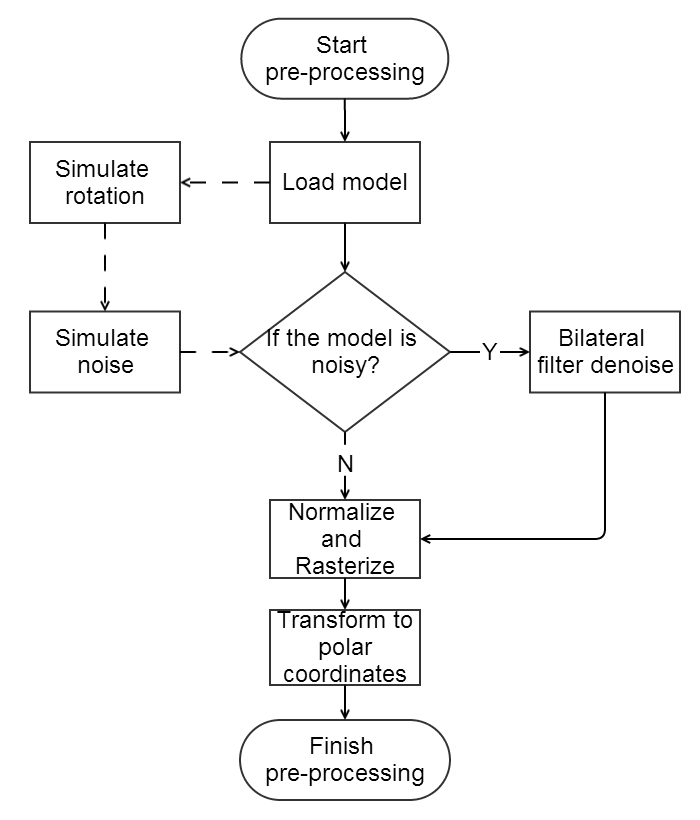
\includegraphics[width=0.5\linewidth]{scan2search_preprocessing}
\caption{Pre-processing of the input model} \label{scan2search_preprocessing}
\end{figure}

The flowchart for the main retrieving process is in Figure~\ref{scan2search_main}. If it is the first time to use the retrieval system, the database for the descriptors should be created. A batch descriptors transformation is required. Every model in the model database will be put into the system, and with the pre-processing steps and spherical harmonics/distance histogram computation, the descriptors database can be generated. With the descriptors' database, and the new descriptors for the input model, the system will compute the similarities between input data and database data. The similarity is simply the Euclidean distance between
descriptors. Besides, since there are two descriptors (spherical harmonics and distance histogram), the result similarities for each of the descriptors will be normalized and combined with weights, which is normally set as 0.5. That is to say, normally the two descriptors are considered to have same weight on the final similarity.

\begin{figure}[h]
\centering
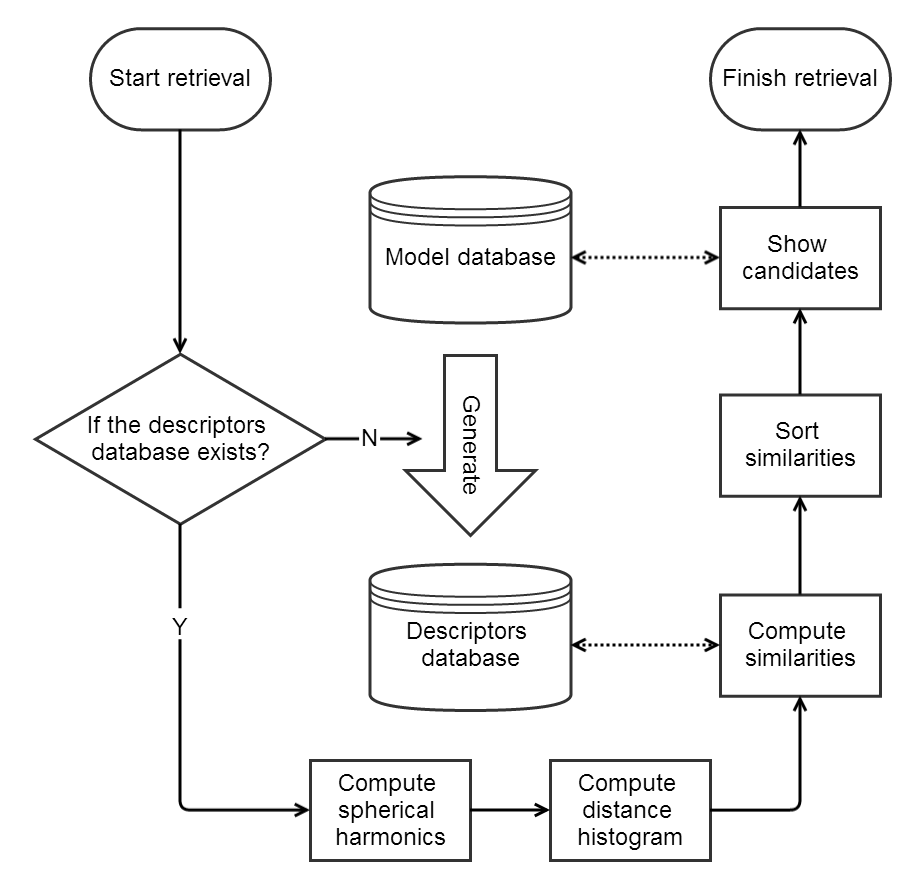
\includegraphics[width=0.4\linewidth]{scan2search_main}
\caption{Retrieval process} \label{scan2search_main}
\end{figure}

The final user interface for the retrieval system is shown in Figure~\ref{UI}. It can be noticed that each processing step is controlled by relevant button. This design allows manual operations so that to observe the intermediate changes and output on each step. In this way, protential errors can be noticed and avoided. After finishing the testing, the user can choose automatically processing and retrieve.

\begin{figure}[h]
\centering
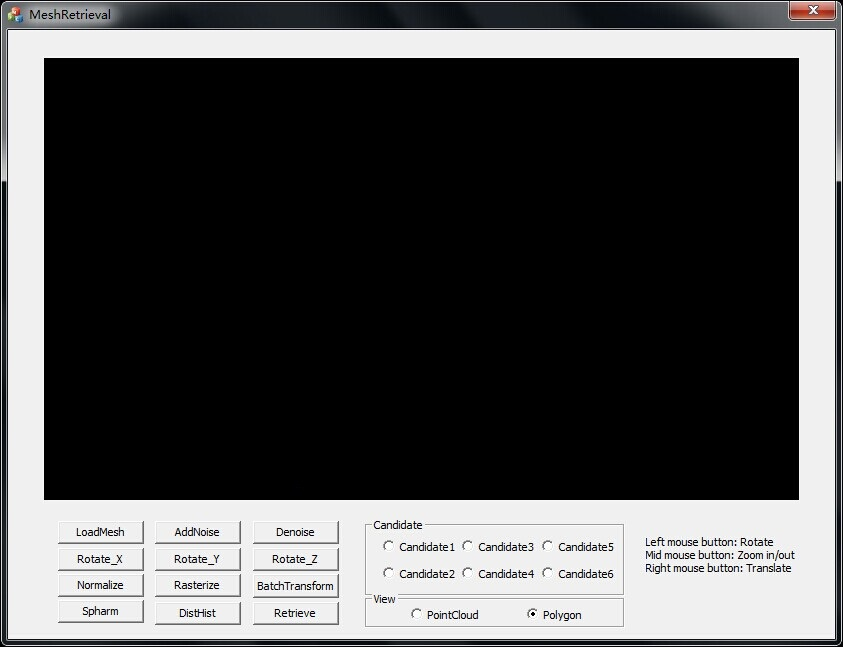
\includegraphics[width=0.7\linewidth]{UI}
\caption{User Interface} \label{UI}
\end{figure}

\section{The final design} \label{sec:thefinaldesign}

At the begining, there is only one spherical harmonics descriptors applied in the system. However, due to some unknown error in the final descriptors (maybe it is the rasterization error or sampling error in the spherical harmonics transformation), there are sometimes some outliers in the output candidate models, whose shapes are not similar to the input data. For example, with the input model(Figure~\ref{input_initialdesign}), the retrieval result shows six candidates in Figure~\ref{output_initialdesign}. It can be observed that some outlier candidates with unsimilar shapes are demonstrated. 


\begin{figure}[h]
\centering
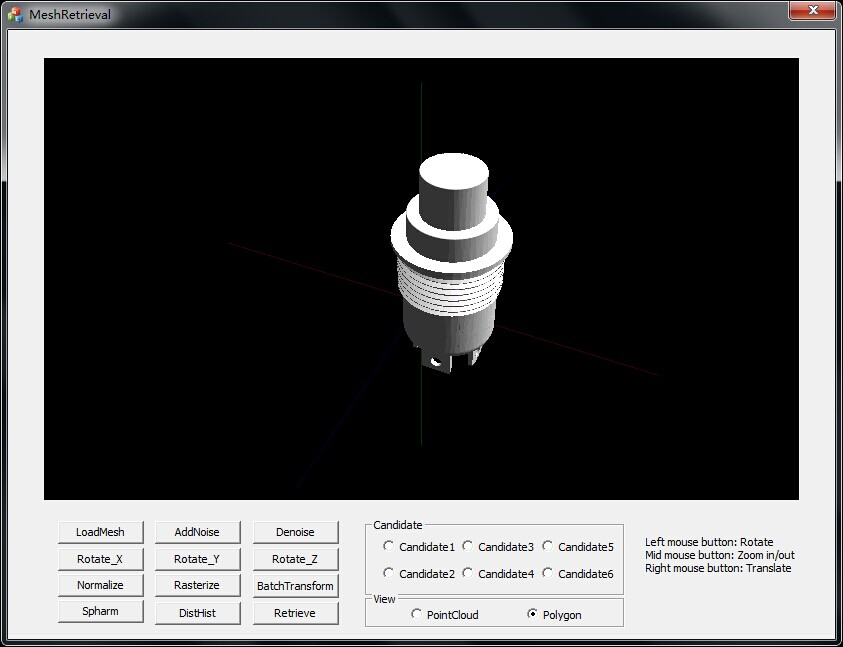
\includegraphics[width=0.7\linewidth]{input_initialdesign}
\caption{Input of the initial design} \label{input_initialdesign}
\end{figure}

\begin{figure}[h]
\centering
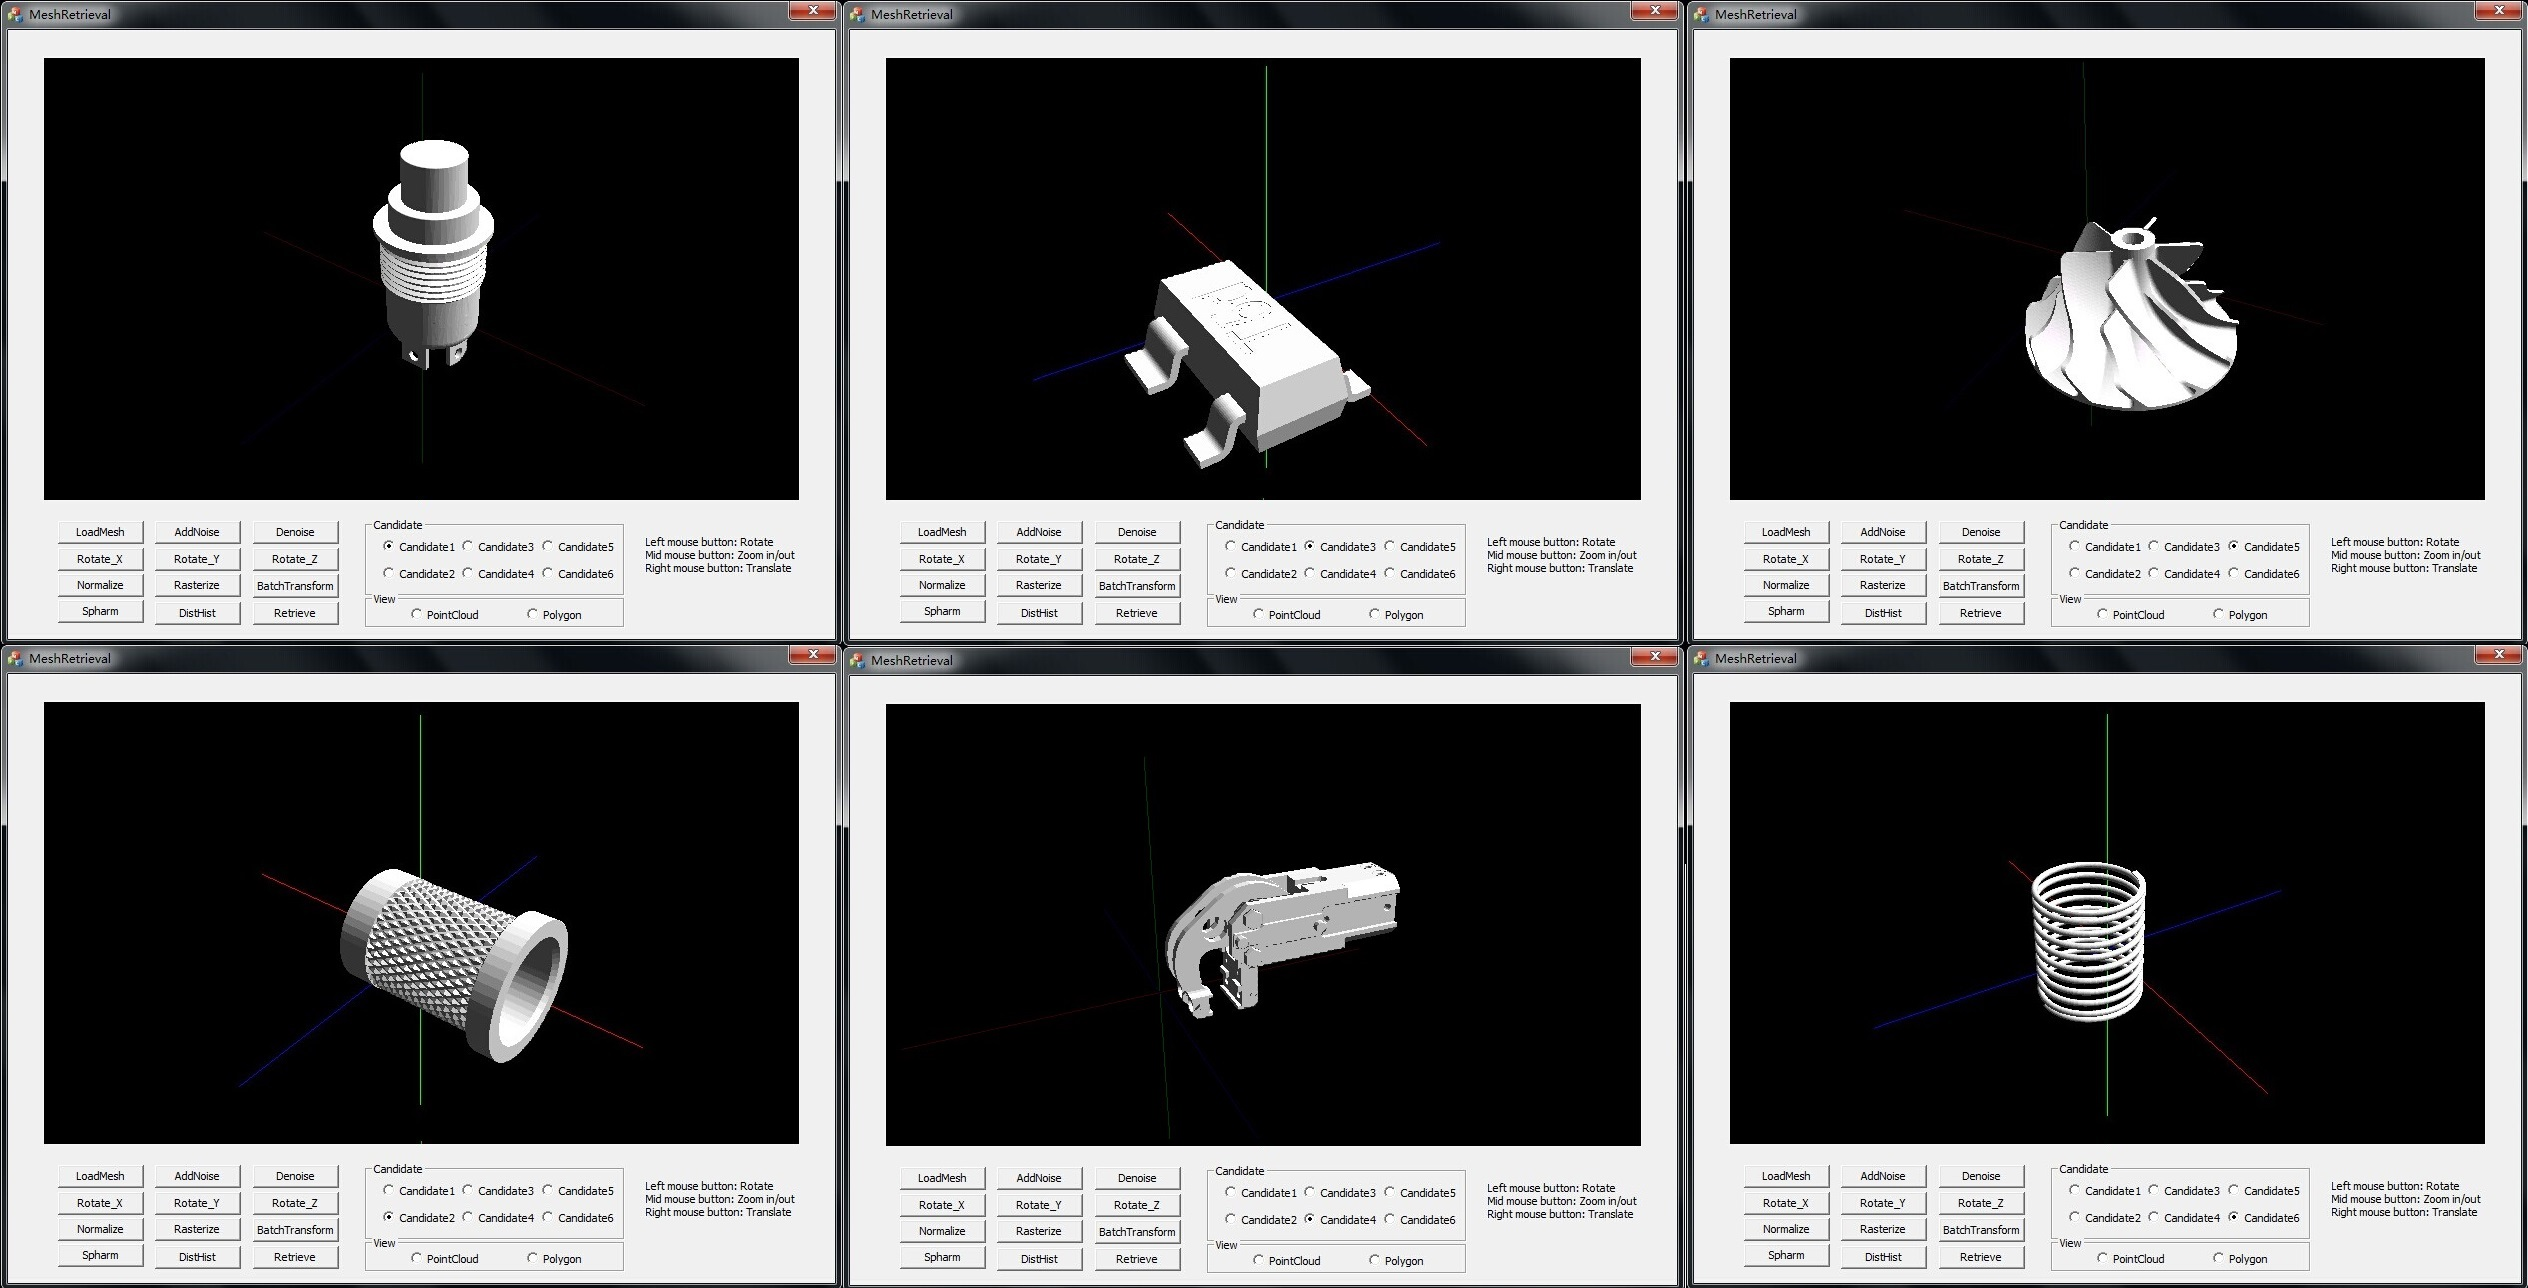
\includegraphics[width=0.7\linewidth]{output_initialdesign}
\caption{Output of the initial design} \label{output_initialdesign}
\end{figure}

Therefore, another simpler distance histogram  descriptors are added. The matching results combine the similarities computed by distance histogram and spherical harmonics, and reduce matching errors. Figure~\ref{output_finaldesign} demonstrates the results of the final design with the same input model. 
\begin{figure}[h]
\centering
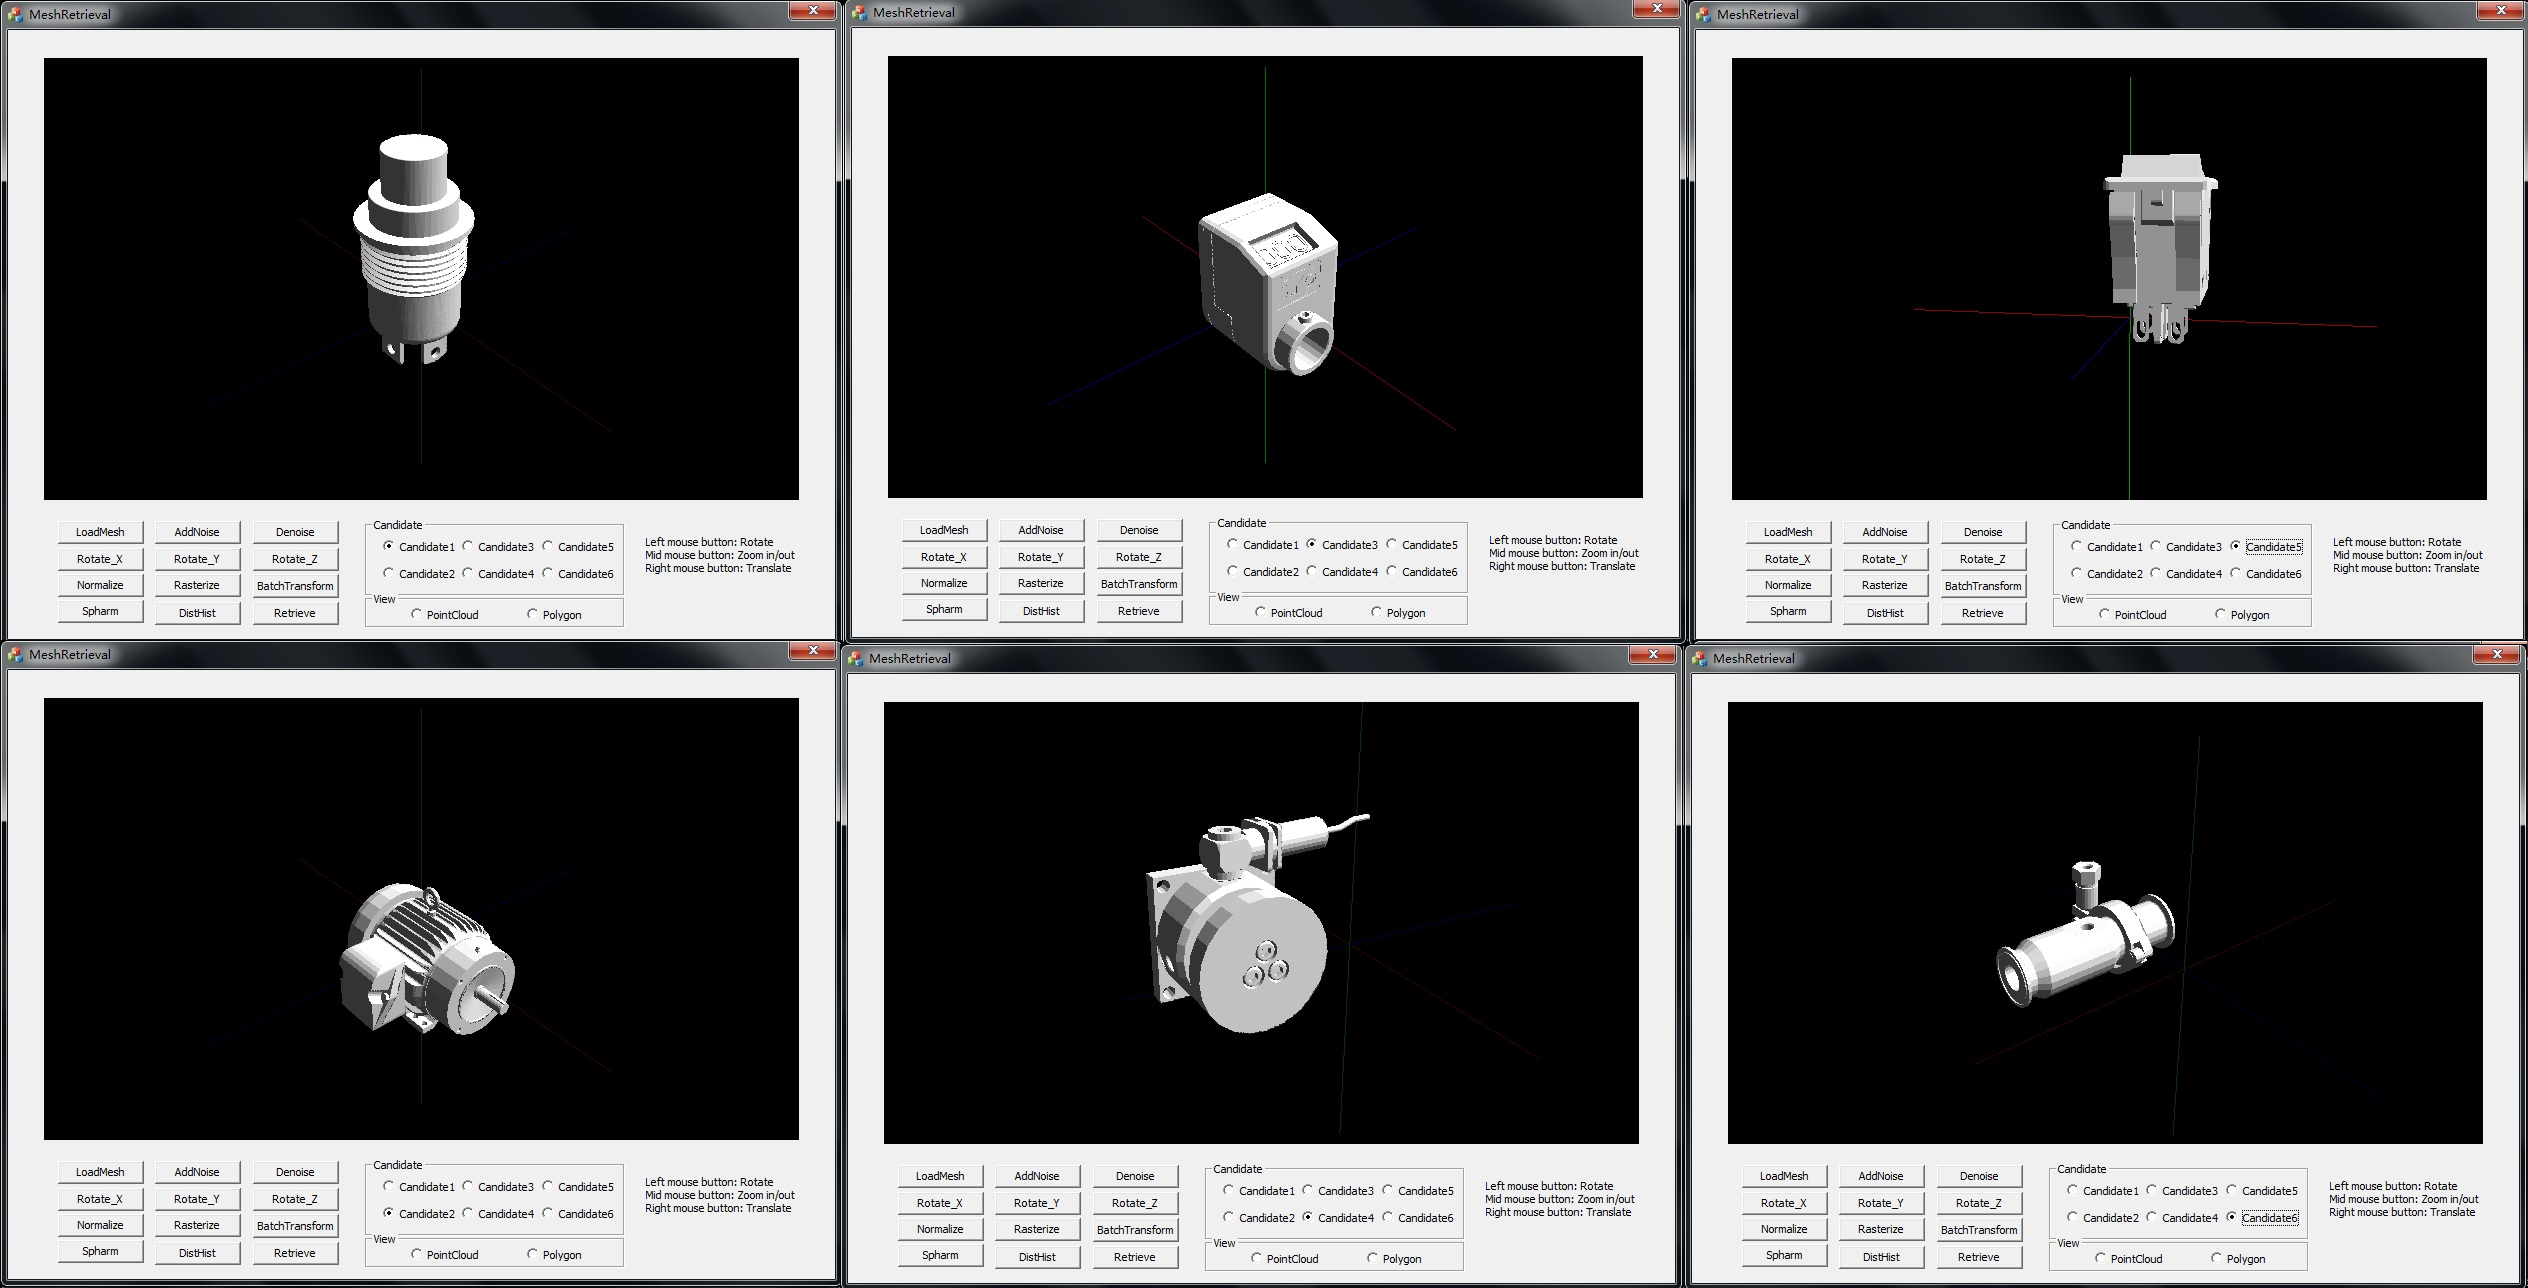
\includegraphics[width=0.7\linewidth]{output_finaldesign}
\caption{Output of the final design} \label{output_finaldesign}
\end{figure}

The verification also worths mentioning. Well designed tests can verify the correctness of the system design and implementation, also they can help to avoid potential risks for further implementation. 

The initial design only has the spherical harmonics descriptors. And spherical harmonics transformation is difficult to implemented. At first the transformation is implemented incorrectly, nevertheless the descriptors can be computed. And even test one ``Retrieval test'' passes. That is because the incorrect descriptors show some features, to some extent. However, the rotational invariance test does not pass, due to the wrong spherical harmonics decomposition. Thus the spherical harmonics decomposition is reimplemented and tested. 

Additionally, after trying larger database with size 60, the output shows the weakness and inaccuracy of single type of descriptors. Therefore another distance histogram matching algorithm is added for assistance.

\chapter{Implementation}
\label{chp:impl}
Since this retrieval system is designed as a loosely coupled system, every basic module can be controlled by its relevant function, and be tested and verified independently. These basic function modules are: load 3D model, add noise, denoise, rotate model, normalize model, rasterize model, compute spherical harmonics, compute distance histogram, batch transformation to generate database, retrieve model, show candidates model after retrieval and show point-cloud/polygon. 

\section{Noise and rotation simulations}

Besides with the function to load 3D models of multiple formats, simulators for noise and rotation are the first important modules to implement. These simulators can help to verify the rotation invariant property of the descriptors, as well as robustness to random noise in the early stage.

Gaussian noise is used for noise simulation. The default standard deviation for Gaussian noise in this module is 0.01. That is for one click on the button ``AddNoise'', the noise with 0.01 standard deviation will be generated and added for every vertex in the 3D model. This function is for simulating scanning noise, the noise intensity can be controlled by the times of click. 

The other function is to rotate the input 3D model. Following Equation~\ref{rotationmatrix_x}, Equation~\ref{rotationmatrix_y} and Equation~\ref{rotationmatrix_z}, basic rotations are applied to the input 3D model to test rotational invariance property. These three basic rotations are controlled by three button ``Rotate\_X'', ``Rotate\_Y'' and ``Rotate\_Z'' respectively. 

\begin{equation} \label{rotationmatrix_x}
  \mathcal{R}_x(\theta_x)=
  \begin{bmatrix}
    1 & 0 & 0 \\
    0 &  \cos{\theta_x} &  -\sin{\theta_x} \\
    0 &  \sin{\theta_x} & \cos{\theta_x}
  \end{bmatrix}
\end{equation}

\begin{equation} \label{rotationmatrix_y}
  \mathcal{R}_y(\theta_y)=
  \begin{bmatrix}
    \cos{\theta_y} & 0 & \sin{\theta_y} \\
    0 & 1 & 0 \\
     -\sin{\theta_y} & 0 & \cos{\theta_y}
  \end{bmatrix} 
\end{equation}

\begin{equation} \label{rotationmatrix_z}
  \mathcal{R}_z(\theta_z)=
  \begin{bmatrix} 
    \cos{\theta_z} &   -\sin{\theta_z} & 0 \\
    \sin{\theta_z} & \cos{\theta_z} & 0 \\
    0 & 0 & 1 
  \end{bmatrix}
\end{equation}

\section{Denoising}

Fleishman~\etal~\cite{fleishman2003bilateral} have proposed a bilateral filter in 3D mesh for denoising. For each vertex in the 3D model, the bilateral filter takes the projections of neighbours onto its normal, as well as the distance to its neighbours into account for smoothing. Therefore it is able to preserve edges while smooth fluctuations for each vertex. 

Let $\bm{\mathrm{u}}=(x,y,z)$ denote one vertex in the mesh, $N(\bm{\mathrm{u}})$ denote the neighbours of $\bm{\mathrm{u}}$. The bilateral filter can be expressed as
\begin{equation} \label{bilaterialfilter}
I^\text{filtered}(\bm{\mathrm{u}}) = \frac{1}{W} \sum_{\bm{\mathrm{p}} \in N(\bm{\mathrm{u}})} I(\bm{\mathrm{p}})W_c(\|\bm{\mathrm{p}}-\bm{\mathrm{u}}\|)W_s(\|I(\bm{\mathrm{p}})-I(\bm{\mathrm{u}})\|),
\end{equation}

where the normalization term
\begin{equation} \label{normalizer}
W = \sum_{\bm{\mathrm{p}} \in N(\bm{\mathrm{u}})}W_c(\|\bm{\mathrm{p}}-\bm{\mathrm{u}}\|)W_s(\|I(\bm{\mathrm{p}})-I(\bm{\mathrm{u}})\|)
\end{equation}.

$W_c$ is the spatial kernel for smoothing differences in distances, and it is a Gaussian function with parameter $\sigma_c$: $W_c=e^{-\frac{x^2}{2 \sigma_c^2}}$, where $\sigma_c$ depends on the average distance of the vertices. Its default value is 0.05. $W_s$ is the range kernel for smoothing differences in the projections of neighbours onto the vertex's normal. $W_s$ is also a Gaussian function with parameter $\sigma_s$: $W_s=e^{-\frac{x^2}{2 \sigma_s^2}}$, where $\sigma_s$ can be computed as the standard deviation of the projections of neighbours onto the vertex's normal. 

The core part of the bilateral filter denoising function is demonstrated in the code below:
%CODE:bilateral filter
\begin{lstlisting}[xleftmargin=1em]
//sigma_c depends on the distance of the points
double sigma_c = 0.05; 
//Calculate sigma_s
mean_height /= neighbour_num;
for(int i=0;i<neighbour_num;i++)
{
	sigma_s +=  pow((height.at(i)-mean_height),2);
}
sigma_s = sqrt(sigma_s);

//Bilateral Mesh Denoising
double sum = 0;
double normalizer = 0;
double t,Wc,Ws;

for(int i=0;i<neighbour_num;i++)
{
	//get distance
	t = distVector.at(i);
	//get Wc, Ws, sum, normalizer
	Wc = exp(-t*t/(2*sigma_c*sigma_c));
	Ws = exp(-height.at(i)*height.at(i)/(2*sigma_s*sigma_s));
	sum += (Wc*Ws)*height.at(i);
	normalizer += Wc*Ws;
}

//assign back to original mesh
for(int d=0;d<dim;d++){
	//new_v = v-n*(sum/normalizer)
	*(mesh.point(it).data()+d) +=-(*(mesh.normal(it).data()+d))*float(sum/normalizer);
}
\end{lstlisting}

When implementing the bilateral filter, it is critical to find the one-ring neighbours for each vertex. However, using the OpenMesh member function and ``VertexVertexIter'' iterator for one-ring neighbours is not efficient. It is caused by the data structure of mesh elements (vertices, half-edges, faces). Because the vertex in the mesh is stored as list, for each vertex it has a slow traversal through the list. The computational complexity for one-ring neighbours is $O(n^2)$. 

Therefore a kd-tree is built to get several nearest neighbours. And some outliers are filtered out, so that to approximately get the one-ring neighbours for further denoising. To build the kd-tree, all the vertices need to be traversed. Its computational complexity is $O(n)$. To find nearest neighbours, the computational complexity is $O(nlog(n))$. Thus With the kd-tree the computational complexity can be reduced to $O(n)+O(nlog(n))$.

To filter out the outliers, the maximum distance between the neighbours and the vertex is acquired. Then a threshold is set according to the maximum distance. If the distance of the neighbour vertex exceeds the threshold, this neighbour vertex will be rejected. The following code shows the implementation:

%CODE:nearest neighbour
\begin{lstlisting}[xleftmargin=1em]
/*find nearest neighbour with kd-tree */
	kdTree->annkSearch(		// search
		Pt,					// query point
		neighbour_num,      // number of near neighbors
		nnIdx,				// nearest neighbors (returned)
		dists,				// distance (returned)
		eps);				// error bound

	//radius = max(dist)
	for (int i=0;i<neighbour_num;i++)
	{
		if(*(dists+i)>radius)	radius = *(dists+i); 
	}
	radius /= 0.9; //reject outliers

	for(int i=0;i<neighbour_num;i++)
	{
		if(*(dists+i)<radius)
		{
			ANNpoint current_neighbour;
			MyMesh::Point  neighbourPt;
			current_neighbour = annAllocPt(dim);

			current_neighbour = meshArray[*(nnIdx+i)];
			neighbourPt.data()[0] = double(current_neighbour[0]);
			neighbourPt.data()[1] = double(current_neighbour[1]);
			neighbourPt.data()[2] = double(current_neighbour[2]);
			neighbours.push_back(neighbourPt);
			distVector.push_back(*(dists+i));
		}
	}
\end{lstlisting}

Lastly, the bilateral filter of 3D mesh may cause mesh shrinkage. This can be overcame by the next module: normalization. 

\section{Rasterization and normalization}

Rasterization and normalization are the pre-processing steps. Rasterization is to sample the 3D model into voxel grids. It can filter out high frequency noise, and meanwhile keep the granularity of the 3D shape. Normalization can make sure the final matching algorithm will not be affected by the scale of the model. The influence of outliers will also be reduced. 

To rasterize, a $2R\times2R\times2R$ voxel grid is created, where $R$ is normally set as 32 for keeping the granularity and filtering out noise. Ideally, a voxel will be assigned a value of 1 (or true) if this voxel touches the surface of the model. But, the data of the 3D model is normally stored in a point cloud. Therefore a important task for rasterization is to find a way to fill the surfaces of the model. 

Face iterator can be used to get vertices for each surface. Since the vertices is in three dimension, it is still difficult to find which voxel is touched by the surface. However, to fill voxels between two vertices is easy. Therefore an idea is try to reduce the dimension, and fill voxels in two dimension. The solution is firstly divide the surface into triangles. With three vertices in one triangle, voxels on two edges can be filled. Then with the help of these voxels, voxels inside the triangle can also be filled. Figure~\ref{rasterization} illustrates the way to fill voxels on edges and then fill voxels in the triangle. Figure~\ref{rasterization_demo} demonstrates the result of rasterization of a 3D model.

\begin{figure}
\begin{center}
\begin{tabular}{cc}   % The "|" bar puts a bar in the figure
   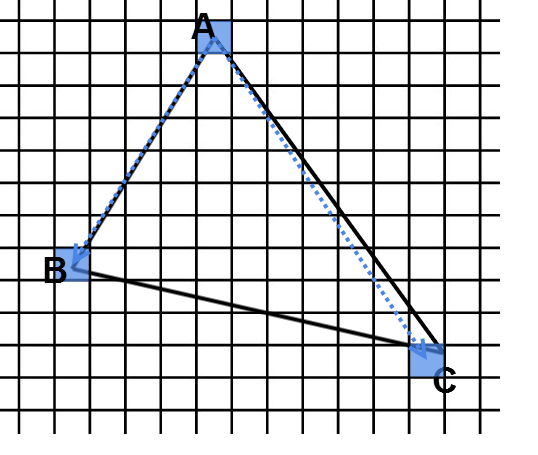
\includegraphics[width=0.45\linewidth]{rasterization_fill2vertices} & 
   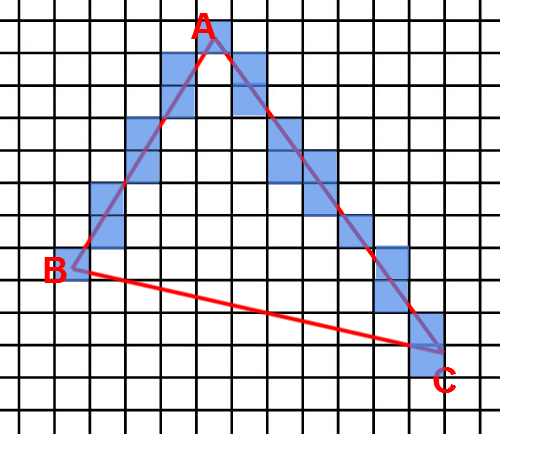
\includegraphics[width=0.45\linewidth]{rasterization_filledges}  \\
   (a) & (b)\\
   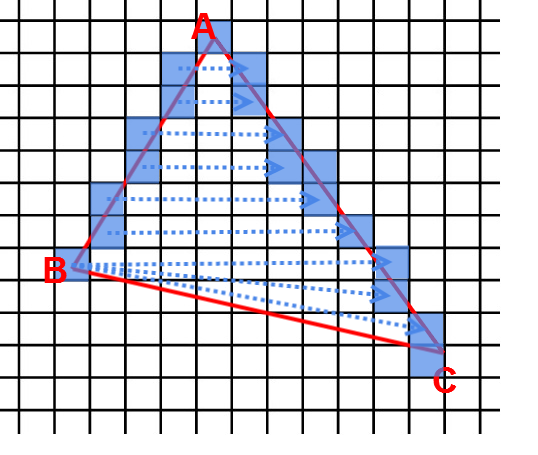
\includegraphics[width=0.45\linewidth]{rasterization_fillsurface} &
   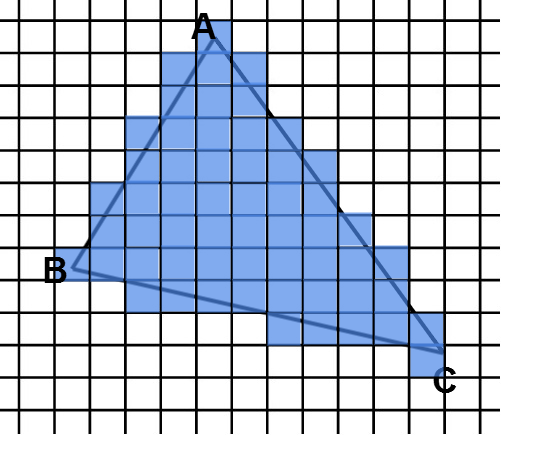
\includegraphics[width=0.45\linewidth]{rasterization_fullfilled}  \\
   (c) & (d)\\
\end{tabular}
\caption{Surface Rasterization: (a) and (b): Fill voxels on edges AB and AC. (c) and (d): With the help of voxels on edges AB and AC, fill voxels inside the triangle.} 
  \label{rasterization}
\end{center}
\end{figure}

\begin{figure}
\begin{center}
\begin{tabular}{ccc}   % The "|" bar puts a bar in the figure
   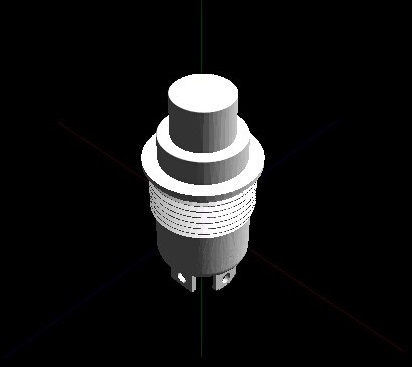
\includegraphics[width=0.3\linewidth]{rasterization_demo1} & 
   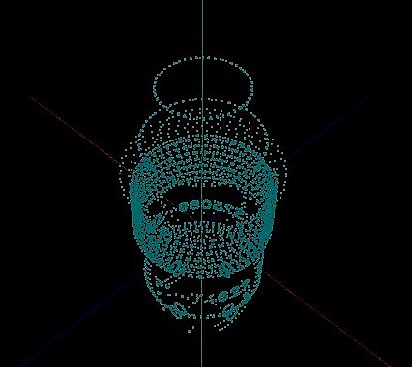
\includegraphics[width=0.3\linewidth]{rasterization_demo2} &
   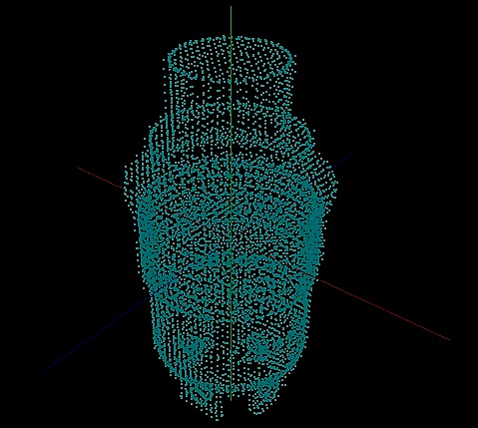
\includegraphics[width=0.3\linewidth]{rasterization_demo3} \\
   (a) & (b) & (c)\\
\end{tabular}
\caption{Rasterization: (a) Model in polygon-mode (b) Model in point-cloud-mode (c) The result of rasterization} 
  \label{rasterization_demo}
\end{center}
\end{figure}

To fill voxels between two vertices is not difficult. Firstly compute the normalized vector between these two vertices. Then start from one vertex and go along with the direction of the vector and fill voxels. The code is demonstrated as below:

\newpage

%CODE:rasterization between two vertices
\begin{lstlisting}[xleftmargin=1em]
/* fill voxels(grid) between two vertices */
Vector v12 = point2-point1;
double len12 = v12.norm();
v12.normalise();

int n_points = 0;
for(unsigned int n=0;n<=floor(len12);n++)
{
    //go along with the direction of the vector and fill voxels
	Point temp_p;
	temp_p.x() = round(point1.x()+v12.x()*double(n));
	temp_p.y() = round(point1.y()+v12.y()*double(n));
	temp_p.z() = round(point1.z()+v12.z()*double(n));

	int grid_coordinate	= int(temp_p.x()*2*RADIUS*2*RADIUS + temp_p.y()*2*RADIUS + temp_p.z());

	//discard outliers
	if(grid_coordinate>(2*RADIUS*2*RADIUS*2*RADIUS-1) || grid_coordinate<0)  continue; 

	if(*(grid+grid_coordinate)!=true)
	{
		*(grid+grid_coordinate) = true;
		inter12.push_back(temp_p);
		grid_points.push_back(temp_p);
		n_points++;
	}
}

//fill the remaining voxels
int grid_coordinate_p2 = int(point2.x()*2*RADIUS*2*RADIUS + point2.y()*2*RADIUS + point2.z());
//make sure points in the range
if(grid_coordinate_p2<(2*RADIUS*2*RADIUS*2*RADIUS-1) && grid_coordinate_p2>0){
	if(*(grid+grid_coordinate_p2)!=true)
	{
		*(grid+grid_coordinate_p2) = true;
		inter12.push_back(point2);
		grid_points.push_back(point2);
		n_points++;
	} 
}
\end{lstlisting}

With $R = 32$, the size of the voxel grid is $2R\times2R\times2R = 262144$, which may occupy a huge memory space. So it is necessary to find a method, which can both save memory and compress the computational complexity. One approach is to create a temporary bitmap (bitset or boolean array in C++) of length $2R\times2R\times2R$ to record whether a voxel is filled. Each element of this bitmap can only show 1 or 0 (true or false), so that the whole bitmap will not occupy any redundant space. While in one traversal($O(n)$) of surfaces of the model, the voxel grid will be filled and the grid vertices should be stored. The pseudocode shows this approach: 

%fill voxel grid
\begin{lstlisting}[xleftmargin=1em]
/* fill voxel grid and get rasterized points in O(n) */

bitmap = new bitmap(2R*2R*2R)               //temporary bitmap
for each voxel to be filled
    if(bitmap(voxel.x,voxel.y,voxel.z))==0  //has not been filled
        bitmap(voxel.x,voxel.y,voxel.z)=1
        grid_point.push_back(voxel)
    end
end
delete bitmap;
\end{lstlisting}

The second pre-processing step is normalization. To normalize, the first step is to compute the center of mass. Then the average distance should be computed and the proportion of the average distance and $R$ can be acquired. Afterwards every vertex is scaled so that the average distance from voxels to the center of mass is $ \frac{R}{2}$. While normalizing, the center of mass will be moved to the origin. This helps further computation of spherical harmonics and distance histogram descriptors.

\section{Rotation invariant descriptors}

Both spherical harmonics descriptors and distance histogram descriptors are rotation invariant descriptors. So these two descriptors can be combined for retrieval. 

\subsection{Spherical harmonics descriptors}

Before carrying out spherical harmonics transformation, the rasterized grid voxels should be transformed to polar coordinates as $f(r,\theta,\phi)$, and sorted according to their distances to the center of mass. A class for polar points is implemented. Its operator $<$ and $>$ are overloaded for suiting the STL sorting algorithm. 

As the radius range is from 0 to 32, the polar points can be divided and form a set ${\left\{ f_0,f_1,...,f_R \right\}}$, with 
\begin{equation}
f_r(\theta,\varphi)=f(r,\theta,\phi).
\end{equation}
Spherical harmonics decomposition can be applied for each $f_r(\theta,\phi)$, so that
\begin{equation}
f_r(\theta,\varphi)=\sum_{l=0}^{\infty}\sum_{m=-l}^{m=l}a_{lm}Y_{l}^{m}(\theta,\varphi),
\end{equation}
where
\begin{equation}
Y_\ell^m( \theta , \varphi ) = (-1)^m \sqrt{{(2\ell+1)\over 4\pi}{(\ell-m)!\over (\ell+m)!}} \, P_\ell^m ( \cos{\theta} ) \, e^{i m \varphi }.
\end{equation}
But the frequency $l$ goes to infinite. It is not able to implement. So it is restricted and a cutoff frequency is set as 32. The decomposition is 
\begin{equation}
f_r(\theta,\varphi)=\sum_{l=0}^{32}\sum_{m=-l}^{m=l}a_{lm}Y_{l}^{m}(\theta,\varphi).
\end{equation}

Details of spherical harmonics decomposition can be seen in Section~\ref{computational_techniques}. For each frequency $l$ and each radius range $r$, the energy can be computed as the $L_{2}$-$norm$ of $a_{lm}$. Let $E_{lr}$ denote the energy in frequency $l$ and radius $r$, we have
\begin{equation}
E_{lr}=\sum_{m=-l}^{m=l}\|a_{ml}\|^{2}.
\end{equation}
The energy is rotation invariant. Therefore spherical harmonics descriptors $SH$ are able to acquire,
\begin{equation}
SH(l,r) = E_{lr}.
\end{equation}

Since with all the coefficients $a_{lm}$, the spherical function $f(\theta,\varphi)$ can perfectly reconstructed. Therefore, the energy of the sum of the coefficients $a_{lm}$ can represent the feature of the spherical function $f(\theta,\varphi)$. Moreover, the spherical harmonics $SH$ is the collection of the energies $E_{lr}$. Thus it can represent the shape feature of the 3D model. 

The pseudocode for spherical harmonics descriptors:

%PSEUDOCODE:spherical harmonics
\begin{lstlisting}[xleftmargin=1em]
/* spherical harmonics descriptors */

for each frequency l
    for each rasterized vertex in one radius range r 
        calculate F_lr = F(l,r)
    end
    a_ml = sum of F_lr in one radius ragion
    SH(l,r) += abs(a_ml)^2    
end
SH = sqrt(SH)
\end{lstlisting}

The code for spherical harmonics descriptors:

%CODE:spherical harmonics
\begin{lstlisting}[xleftmargin=1em]
/* spherical harmonics descriptors */

int idx_n = 0;
double *SH_descriptor;
SH_descriptor = new double [MAX_R*MAX_L]();

for(unsigned int idx_r = 1;idx_r<=RADIUS;idx_r++)
{
	//for each frequency
	for(int idx_l = 0;idx_l<MAX_L;idx_l++)
	{
		vector<double> 	a_ml_pow;
		//traverse frequency range
		for(int idx_m = -idx_l;idx_m<=idx_l;idx_m++)
		{
			vector<double> Yml_real,Yml_imag;
			double NPml;

			while(idx_n<=(grid_polar_points.size()-1) && grid_polar_points.at(idx_n).distance()<idx_r)
			{
				//initial Y_ml = N*P(m,l,cos(theta))*exp(i*m*phi)
				//function gsl_sf_legendre_sphPlm returns value of N*P(m,l,cos(theta))
				//cos(x) input should be a radian
				//theta_vector and phi_vector are radians
				PolarPoint current_p = grid_polar_points.at(idx_n);
				if(idx_m>=0)
				{
					NPml = gsl_sf_legendre_sphPlm(idx_l,idx_m,cos(current_p.theta()));
					Yml_real.push_back(NPml*cos(double(idx_m)*current_p.phi()));
					Yml_imag.push_back(NPml*sin(double(idx_m)*current_p.phi()));
				} else {
					NPml = pow (-1.0,-idx_m)*gsl_sf_legendre_sphPlm(idx_l,-idx_m,cos(current_p.theta()));
					Yml_real.push_back(NPml*cos(double(-idx_m)*current_p.phi()));
					Yml_imag.push_back(NPml*sin(double(-idx_m)*current_p.phi()));
				}
				idx_n++;
				if(idx_n==(grid_polar_points.size()-1)) break;
			}//while(dist_vector.at(idx_n)<idx_r)

			double 	a_ml_real,a_ml_imag;
			a_ml_real=accumulate(Yml_real.begin(),Yml_real.end(),0.0);
			a_ml_imag=accumulate(Yml_imag.begin(),Yml_imag.end(),0.0);
			a_ml_pow.push_back(pow(a_ml_real,2.0)+pow(a_ml_imag,2.0));
			if(idx_l!=MAX_L-1) idx_n-=Yml_real.size();
		}//finish traversing frequency range
		SH_descriptor[(idx_r-1)*MAX_R+idx_l] = sqrt(accumulate(a_ml_pow.begin(),a_ml_pow.end(),0.0));
	}
}

/*write out the data*/
WriteSH(write_filename,SH_descriptor);

delete [] SH_descriptor;
\end{lstlisting}


\subsection{Distance histogram descriptors}

As for the distance histogram descriptors, they are simpler and are used to correct or supplement the spherical harmonics descriptors. First, the center of mass should be acquired. Then for each voxel in the grid, compute its distance to the center of mass. The distance within certain range will be recorded and counted. Lastly, the 
distribution of distances from vertices to the center of mass is acquired. This distribution is just the distance histogram descriptors.  

The core code for distance histogram is as follow: 

%distance histogram
\begin{lstlisting}[xleftmargin=1em]
/* distance histogram descriptors */

//move grid to the origin and get distance vector
double x_dist,y_dist,z_dist;
for(unsigned int p_it = 0;p_it<grid_points.size();p_it++)
{
	x_dist = grid_points.at(p_it).x() - centroid.x();
	y_dist = grid_points.at(p_it).y() - centroid.y();
	z_dist = grid_points.at(p_it).z() - centroid.z();
	int distance = int(round(sqrt(pow(x_dist,2.0)+pow(y_dist,2.0)+pow(z_dist,2.0))));
	DistHist[distance]+=1.0;
}

//normalize histogram
double grid_size = double (grid_points.size());
for(unsigned int d_it=0;d_it<MAX_DIST;d_it++){
	DistHist[d_it]/=grid_size;
}
\end{lstlisting}

\section{Retrieval}

If it is the first time to use the retrieval system, the database for the descriptors should be created. There will be two databases for the retrieval system: one is storing all the 3D models; the other is for storing the relevant descriptors of the models. For creating the descriptors database, a batch descriptors transformation module needs to be implemented. Every model in the model database will be put into the system, and with the pre-processing steps as well as the spherical harmonics/distance histogram computation, the descriptors database can be generated.

With the descriptors for the input model prepared, the similarities between the input model and models in the database are computed. The similarity is simply the Euclidean distance between two descriptors. Since there are two descriptors (spherical harmonics and distance histogram), the result similarities for each of the descriptors will be normalized and combined with weights, which is normally set as 0.5. That is to say, normally the two descriptors are considered to have same weight on the final similarity. After retrieval, six candidate models with high similarities will be demonstrated.  The user can choose to show polygon models or models in point clouds. The latter type can be shown efficiently on the screen, because it does not need shading computation for each surface.  









\chapter{Evaluation}
\label{chp:eval}
%\input{evaluation.tex}


\section{Figures} \label{sectionExample}

Figure~\ref{ExampleEstNoiseCovar}, is an example of a figure with a legend.

\begin{figure}[h]
\centering
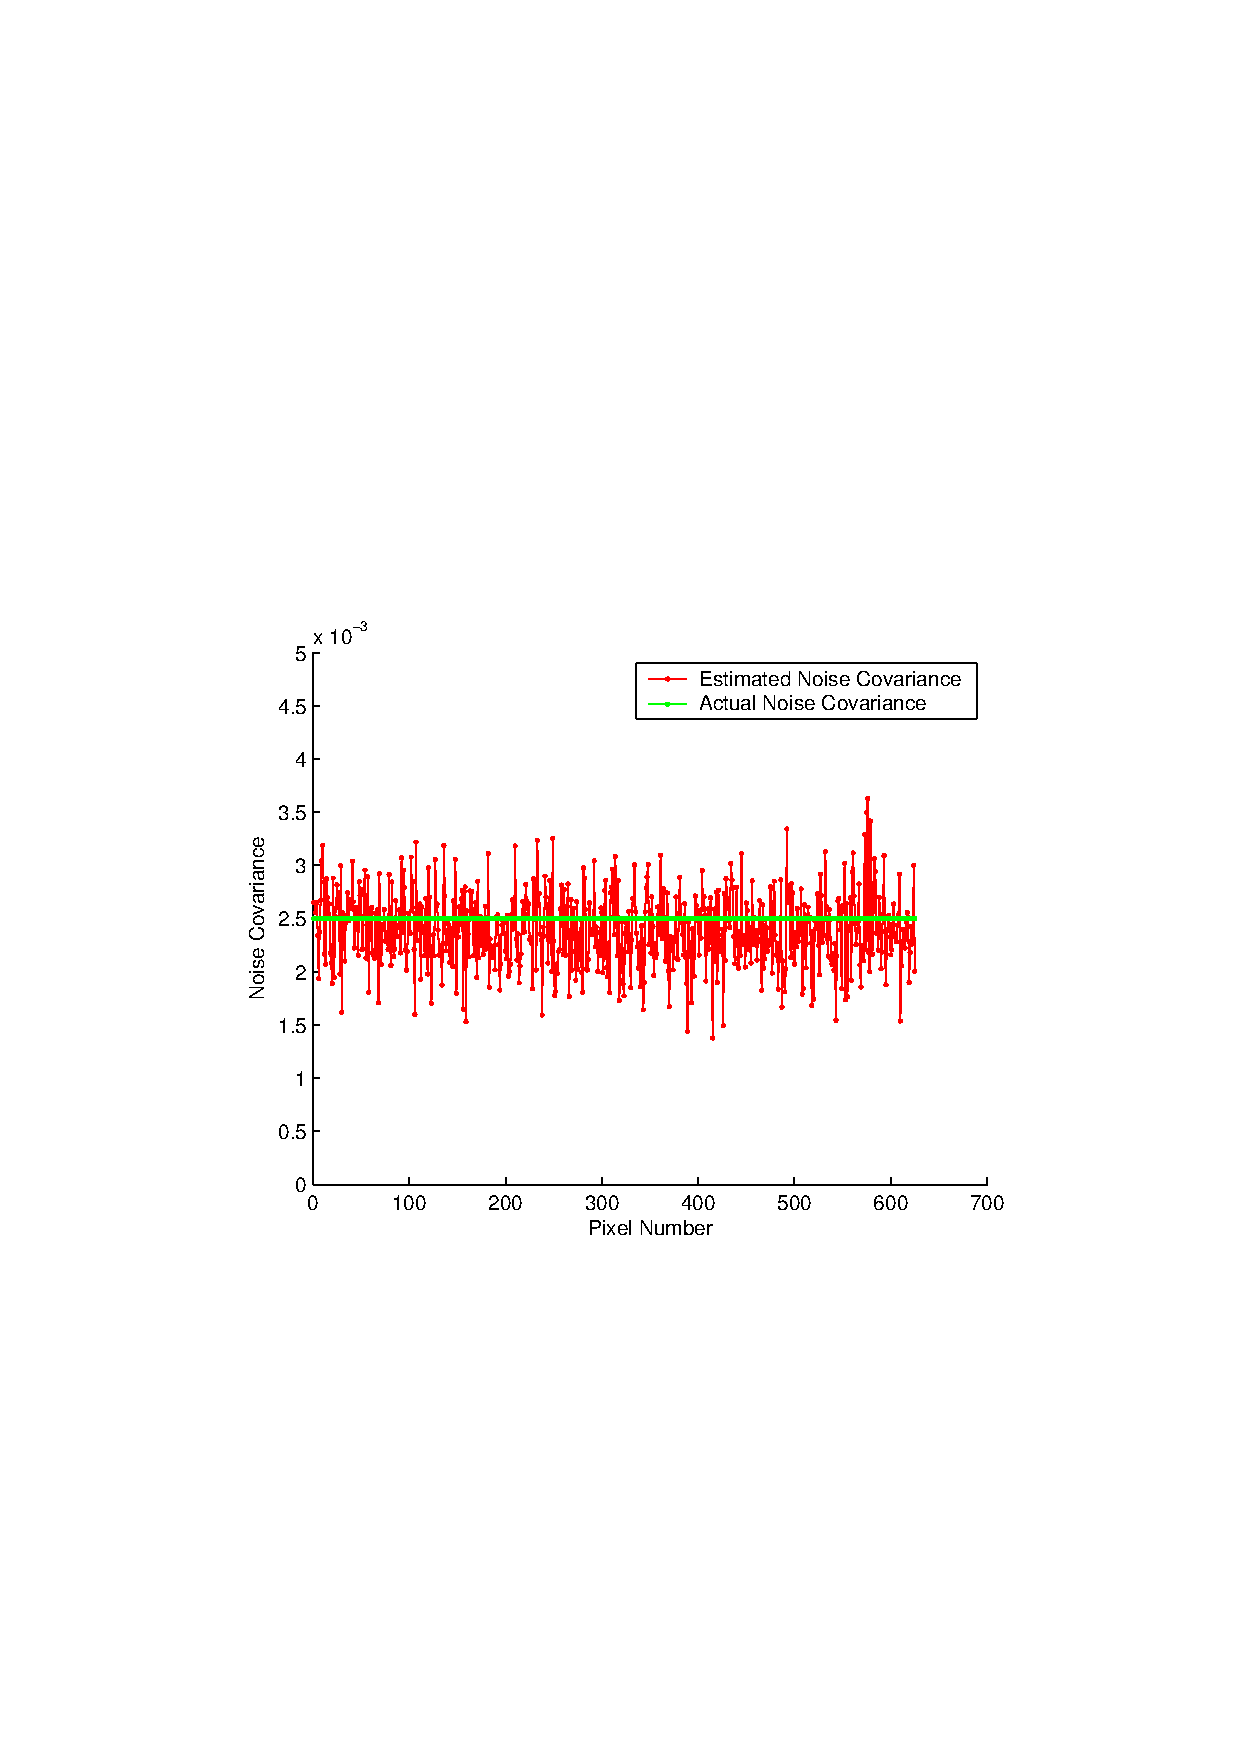
\includegraphics[width=0.5\linewidth]{exampleEstNoiseCovar}
\caption{This is the figure caption. Notice the figure looks good even when magnified because it is a vector-graphic, and not rasterized.} \label{ExampleEstNoiseCovar}
\end{figure}


\textbf{Old and New Instructions} These instructions are partly ``old'' because instead of .eps, we usually put pdf or png figures in our documents these days. However, they're still useful because exporting of Matlab figures directly to pdf, when using the Student License version of Matlab, results in an undesirable watermark. So my advice is to prepare your raster images as .png's, prepare your vector graphics as .pdf's in Inkscape or even Office (with the MS plugin that exports to .pdf), and follow the following slightly roundabout process to get Matlab figures into .pdf form.
\begin{enumerate}
  \item Make the figure in Matlab.
  \item Do \texttt{print -depsc2} to generate an .eps.
  \item Open the .eps in Ghostview (GSview) and ``Convert'' using the ``pdfwrite'' device to save a .pdf.
\end{enumerate}




\chapter{Conclusion}
\label{chp:conc}
%\section{Conclusion}

In summary, this project build a 3D retrieval system which provides a ``scan to search'' solution for manufacturing components. A 3D bilateral filter is applied to reduce the scanning noise. Two types of rotation invariant shape descriptors are combined to describe the shape feature of 3D models. A series of tests indicate that the spherical harmonics shape descriptors can describe the shape feature of the model in detail. However, spherical harmonics may be affected by the sampling error in rasterization of the model. Therefore, the second descriptors distance histogram is used to roughly describe the shape feature again, so that to compensate the potential error of spherical harmonics. 

\section{Future works}

This system can still be improved in many aspects. The following are some topics that worth further investigation.

\begin{enumerate}
\item A better user interface: 

Since this project only implement a prototype retrieval system. The user interface is built in a MFC dialog. The user interface is not that user-friendly. So a better user interface can be built for fast rendering of meshes, as well as better appearance.

\item A fast way to compute spherical harmonics: 

Current spherical harmonics decomposition is time-consuming. A solution is to reduce the cut-off frequency from 32 to 16. However, such approach is just a palliative. A fast way to compute spherical harmonics should be investigated and applied to the system. For example, M. Mousa~\etal~\cite{mousa2006direct} provides a fast and accurate technique for computing spherical
harmonics.

\item New descriptors:

As it is mentioned in the Evaluation section (Section~\ref{sec:results_rotationinvarianttest}), current two types of descriptors (spherical harmonics and distance histogram) cannot detect interior rotation of a model. Thus a new type of descriptors can be created, which has rotation invariant property and will not lost information of interior rotation. 
\item Crawling the web for sizeable database:

Current models in the database are manually collected from the Internet. To build a sizeable database, manual collecting is impractical. Therefore a crawler can be implemented to collect specified manufacturing 3D models.  

\item Accelerating the matching speed in a sizable 3D database: 

Currently this system compute similarity of the query model with all the models in the database. It would be useful to build a high dimensional kd-tree for fast retrieval in a sizable database. 

\item Clustering datasets in the database for fast retrieval and precise presentation of results:

The database can be clustered into small subsets of data with similar shape feature. For example, a subset contains models with cylinder-like shape is built. If the input model is detected as cylinder-like shape, the system can quickly compute its similarity with subsets and find the subset with cylinder-like shape feature. In this way, the retrieval speed is accelerated. Moreover, the presentation of the candidate models would be more accurate, because more weights can be added to the models in the matched subset. This can also help to avoid irrelevant matching results. 

\end{enumerate}

\begin{figure}
\begin{center}
\begin{tabular}{c|cc}   % The "|" bar puts a bar in the figure
   
\includegraphics[width=.30\columnwidth]{home.png} &  % The little "and" puts splits in the table
   
\includegraphics[width=.30\columnwidth]{home.png} &  
   
\includegraphics[width=.30\columnwidth]{home.png}\\
   (A) & (B) & (C)
\end{tabular}
\caption{Another figure caption. These should be meaningful and somewhat self-contained.} 
  \label{fig:SomeMoreFigs}
\end{center}
\end{figure}

Figures need not be in \texttt{.pdf} format. For example, Figure~\ref{fig:SomeMoreFigs} pulls in $3$ copies of a \texttt{.png} file. Also, notice that the automatic-placement of figures will try to put each figure as close as possible to the first reference in the final document, regardless of figure-placement in the .tex.



\addcontentsline{toc}{chapter}{Appendices}

\cleardoublepage
\appendix
\chapter{Theoretical Background}
\label{chp:theory}
%\input{theory.tex}

\chapter{Lisp Primer}
\label{cha:lisp-primer}
%\input{lisp-primer.tex}


\addcontentsline{toc}{chapter}{Bibliography}

\bibliography{Thesis}
\end{document} 